


\begin{frame}{OpenCL Heterogeneity}

 \begin{block}{OpenCL Releases}
   \begin{itemize}
    \item OpenCL 2.2 (recently)
    \item OpenCL 2.1 (2015)
    \item OpenCL 2.0 (2013)
    \item OpenCL 1.2 (2011)
    \item OpenCL 1.1 (2010)
    \item OpenCL 1.0 (2009)
   \end{itemize}
 \end{block}

 %\pause
 \begin{block}{OpenCL Support in SDKs}
   \begin{itemize}
    \item 2.2: -
    \item 2.1: -
    \item 2.0: AMD, Intel (Win), Qualcomm
    \item 1.2: Apple, Beignet, Intel (Linux), Imagination, NVIDIA, pocl, Vivante
    \item 1.1: ARM, Sony, TI
    \item 1.0: Altera, Xilinx
   \end{itemize}
 \end{block}
 
\end{frame}



\begin{frame}{OpenCL Heterogeneity}

 \begin{block}{The Veto Problem}
   \begin{itemize}
    \item What if a major vendor stops OpenCL SDK development?
    \item What if SPIR-V is not broadly available?
   \end{itemize}
 \end{block}

 %\pause
 \begin{block}{Possible Reasons for Slow OpenCL SDK Development}
   \begin{itemize}
    \item Proprietary alternative available
    \item ``Will help competitor more than us''
    \item Development too expensive
   \end{itemize}
 \end{block}
 
\end{frame}
% 


\begin{frame}{OpenCL Heterogeneity}

 \begin{block}{How to Encourage?}
 \end{block}

 %\pause
 
 \begin{center}
  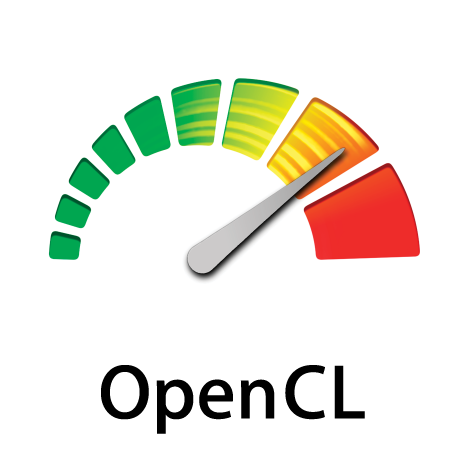
\includegraphics[width=0.2\textwidth]{figures/opencl} \ \ \ \ 
  
\includegraphics[width=0.5\textwidth]{figures/vulkan-logo}\\[1.5em]
  Make OpenCL a prerequisite for Vulkan certification?
 \end{center}
 
\end{frame}
